\documentclass[11pt,a4paper]{article}

\usepackage{fontspec}
\usepackage[vietnamese]{babel}
\setmainfont{Times New Roman}

\usepackage[a4paper,margin=2cm]{geometry}
\usepackage{graphicx}
\graphicspath{{../../assets/diagrams/}}
\usepackage{longtable}
\usepackage{tabularx}
\usepackage{array}
\usepackage{enumitem}
\usepackage{needspace}
\usepackage{xcolor}
\usepackage{tikz}
\usetikzlibrary{arrows.meta,positioning,fit,calc}
\usepackage{listings}
\usepackage{caption}
\usepackage{hyperref}
\usepackage{fancyhdr}
\usepackage{csquotes}
\DeclareQuoteStyle{vietnamese}
  {\textquotedblleft}{\textquotedblright}{\textquoteleft}{\textquoteright}
\usepackage[backend=biber,style=numeric,sorting=none]{biblatex}
\DeclareLanguageMapping{vietnamese}{english}
\DeclareFieldFormat{urldate}{%
  \mkbibparens{truy cập ngày\space
  \mkdayzeros{\thefield{urlday}}/\mkmonthzeros{\thefield{urlmonth}}/\thefield{urlyear}}}
\addbibresource{references.bib}
\setcounter{biburlnumpenalty}{100}
\setcounter{biburlucpenalty}{200}
\setcounter{biburllcpenalty}{200}
\AtBeginBibliography{\footnotesize}
\setlength{\bibitemsep}{0.05em}

\definecolor{internallinkblue}{HTML}{0057A8}

\hypersetup{
  colorlinks=true,
  linkcolor=internallinkblue,
  urlcolor=blue,
  citecolor=blue,
  pdftitle={Nghiên cứu .NET Parallel, Background Job và Vue 2},
  pdfauthor={Đặng Phúc An Khang}
}

\newcommand{\figref}[1]{\hyperref[#1]{Hình~\ref*{#1}}}

\lstset{
  basicstyle=\ttfamily\footnotesize,
  breaklines=true,
  columns=fullflexible,
  keepspaces=true,
  frame=single,
  rulecolor=\color{gray!65},
  framerule=0.5pt,
  framesep=5pt,
  numbers=none,
  showstringspaces=false,
  tabsize=2,
  xleftmargin=0.5em,
  xrightmargin=0.5em,
  aboveskip=0.5em,
  belowskip=0.5em
}

\renewcommand{\arraystretch}{1.2}
\setlength{\tabcolsep}{4pt}
\setlist{itemsep=0.2em,topsep=0.3em,leftmargin=*}
\setlength{\parskip}{0.25em}
\setlength{\emergencystretch}{2em}
\captionsetup{
  font=small,
  labelfont=bf,
  labelsep=period,
  justification=centering,
  skip=0.2em,
  hypcap=false
}
\renewcommand{\figurename}{Hình}
\renewcommand{\tablename}{Bảng}

\pagestyle{fancy}
\fancyhf{}
\fancyhead[L]{TASK-001 - BÁO CÁO KỸ THUẬT}
\fancyhead[R]{Đặng Phúc An Khang}
\fancyfoot[C]{\thepage}
\setlength{\headheight}{14pt}
\fancypagestyle{plain}{
  \fancyhf{}
  \fancyhead[L]{TASK-001 - BÁO CÁO KỸ THUẬT}
  \fancyhead[R]{Đặng Phúc An Khang}
  \fancyfoot[C]{\thepage}
  \renewcommand{\headrulewidth}{0.4pt}
}

\fancypagestyle{firstpage}{
  \fancyhf{}
  \fancyfoot[C]{\thepage}
  \renewcommand{\headrulewidth}{0pt}
}

\begin{document}

\thispagestyle{firstpage}
\begin{center}
  {\small\bfseries BÁO CÁO NGHIÊN CỨU KỸ THUẬT\par}
  \vspace{0.25cm}
  {\LARGE\bfseries Parallel và Background Job trong .NET/C\#\par}
  \vspace{0.15cm}
  {\Large Cú pháp và cơ chế hoạt động của Vue 2\par}
\end{center}

\vspace{0.45cm}

\begin{center}
\small
\renewcommand{\arraystretch}{1.22}
\begin{tabularx}{\textwidth}{|>{\bfseries\raggedright\arraybackslash}p{0.18\textwidth}|>{\raggedright\arraybackslash}p{0.25\textwidth}|>{\bfseries\raggedright\arraybackslash}p{0.19\textwidth}|>{\raggedright\arraybackslash}X|}
\hline
Người thực hiện & Đặng Phúc An Khang & Bộ phận & Kỹ thuật \\
\hline
Vị trí & Thực tập sinh Full-stack Developer & Người giao và duyệt & CTO Tín Nguyễn \\
\hline
Thời gian thực hiện & 03/08/2026 - 04/08/2026 & Ngày báo cáo & 04/08/2026 \\
\hline
\end{tabularx}
\end{center}

\vspace{0.35cm}

\section*{Mục tiêu và phạm vi}

Báo cáo trình bày ba nội dung: Parallel (xử lý song song) trong .NET/C\#, Background Job trong
.NET và cú pháp cùng cơ chế hoạt động của Vue 2. Phần .NET tập trung vào cách hoạt
động, trường hợp sử dụng và các thay đổi trực tiếp từ .NET Core 3.1 đến .NET 8.
Phần Background Job ưu tiên cơ chế có sẵn của .NET và đối chiếu ngắn với hai thư viện
quản lý job bên ngoài. Phần Vue 2 giới thiệu cú pháp component và luồng cập nhật giao diện
khi dữ liệu thay đổi.

\section{Khái niệm nền về xử lý công việc}

\subsection{Concurrency, parallelism, bất đồng bộ và Background Job}

\textbf{Thread (luồng thực thi)} là một chuỗi lệnh được CPU thực hiện. Một chương
trình có thể có nhiều thread. \textbf{CPU core (lõi xử lý)} là đơn vị phần cứng có
khả năng thực thi lệnh; nhiều core cho phép nhiều thread thực sự chạy cùng lúc.

\begin{itemize}
  \item \textbf{Concurrency (xử lý đồng thời)} là quản lý nhiều công việc trong cùng
  một khoảng thời gian. Các công việc có thể xen kẽ nhau, chưa chắc chạy đúng cùng
  một thời điểm.

  \item \textbf{Parallelism (xử lý song song)} là nhiều phần tính toán thực sự chạy
  cùng lúc trên nhiều CPU core. Đây là một cách thực hiện concurrency.

  \item \textbf{Asynchronous programming (lập trình bất đồng bộ)} cho phép phương
  thức tạm nhường quyền thực thi trong lúc chờ thao tác vào/ra (I/O) như mạng,
  database hoặc file. Từ khóa \texttt{await} không tự tạo thêm thread; nó giúp
  thread hiện tại quay lại xử lý việc khác cho đến khi thao tác chờ hoàn tất.

  \item \textbf{Background Job (công việc nền)} là công việc chạy độc lập với
  request, tức yêu cầu mà máy khách gửi đến server. Chẳng hạn, job dọn dữ liệu lúc
  nửa đêm có thể tiếp tục sau khi server đã trả phản hồi cho máy khách.
\end{itemize}

\figref{fig:async-io-flow} minh họa điều xảy ra tại \texttt{await}. Phương thức gửi
yêu cầu I/O rồi tạm dừng; thread đang chạy phương thức được trả về ThreadPool để xử
lý việc khác. Khi I/O hoàn tất, phần code sau \texttt{await} được xếp lịch để tiếp
tục thực hiện.

\begin{center}
\resizebox{0.84\textwidth}{!}{\begin{tikzpicture}[
  node distance=8mm and 10mm,
  every node/.style={font=\small,align=center},
  flowbox/.style={draw,rounded corners=2mm,minimum height=11mm,minimum width=28mm,thick},
  arrow/.style={-{Latex[length=2mm]},thick},
  waitarrow/.style={-{Latex[length=2mm]},thick,dashed,draw=gray!75}
]
\node[font=\small\bfseries] (threadlabel) {Thread};
\node[flowbox,fill=blue!15,draw=blue!55,right=of threadlabel] (start) {Bắt đầu\\phương thức};
\node[flowbox,fill=orange!18,draw=orange!70!black,right=of start] (send) {Gửi yêu cầu I/O\\rồi gặp await};
\node[flowbox,fill=green!15,draw=green!55!black,right=of send] (free) {Thread quay lại\\ThreadPool};
\node[flowbox,fill=blue!12,draw=blue!55,right=of free] (resume) {Tiếp tục xử lý\\sau await};

\node[font=\small\bfseries,below=16mm of threadlabel] (iolabel) {I/O};
\node[flowbox,fill=gray!12,draw=gray!65,below=16mm of send] (io) {Mạng, database hoặc file\\thực hiện thao tác};

\draw[arrow] (start) -- (send);
\draw[arrow] (send) -- (free);
\draw[arrow] (send) -- (io);
\draw[waitarrow] (io) -| node[pos=0.72,below,font=\scriptsize] {hoàn tất} (resume);
\end{tikzpicture}
}
\captionof{figure}{Luồng thực thi khi phương thức bất đồng bộ chờ I/O}
\label{fig:async-io-flow}
\end{center}

\figref{fig:concurrency-single-thread} minh họa concurrency trên một thread.
Ba công việc A, B và C đều tiến triển trong cùng một khoảng thời gian, nhưng tại
mỗi thời điểm CPU chỉ thực thi một đoạn của một công việc. Hệ thống chuyển qua lại
giữa các đoạn nên các công việc trông như cùng chạy; đây là sự xen kẽ, chưa phải
parallelism thực sự.

\begin{center}
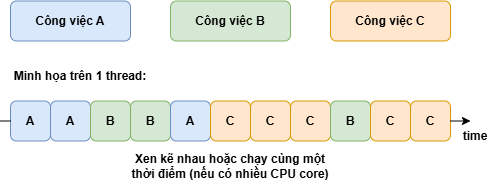
\includegraphics[width=0.64\textwidth]{../../assets/images/concurrency-single-thread.png}
\captionof{figure}{Concurrency trên một thread: các công việc được thực thi xen kẽ}
\label{fig:concurrency-single-thread}
\end{center}

Ngược lại, \figref{fig:parallelism-multiple-cores} minh họa parallelism. Các công
việc A, B và C được thực thi tại cùng một thời điểm trên các CPU core khác nhau.
Vì có nhiều phép tính thật sự diễn ra đồng thời, đây là xử lý song song chứ không
chỉ là chuyển lượt thực thi trên một core.

\begin{center}
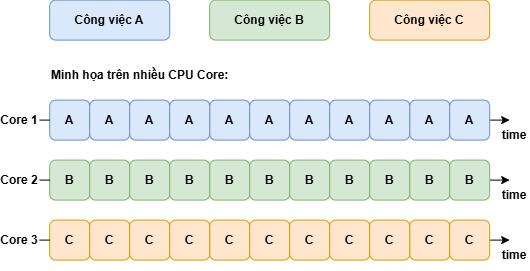
\includegraphics[width=0.64\textwidth]{../../assets/images/parallelism-multiple-cores.png}
\captionof{figure}{Parallelism trên nhiều CPU core: các công việc được thực thi đồng thời}
\label{fig:parallelism-multiple-cores}
\end{center}

Có thể hình dung bằng việc nấu ăn: một người tranh thủ chuẩn bị món khác trong lúc
chờ món đang nấu là async/concurrency; nhiều người cùng nấu các món khác nhau mới là
parallelism. Điểm khác nhau nằm ở việc công việc chỉ được sắp xếp xen kẽ hay thật sự
được thực thi đồng thời trên nhiều tài nguyên.

Trong C\#, \texttt{Task} đại diện cho một thao tác đang thực hiện hoặc sẽ hoàn tất
trong tương lai. Một Task không đồng nghĩa với một thread riêng: thao tác có thể chờ
I/O mà không giữ thread hoặc được thực thi bằng thread do .NET quản lý, tùy theo bản
chất công việc.

\subsection{Phân loại tác vụ theo tài nguyên giới hạn}

\textbf{CPU-bound} nghĩa là tốc độ bị giới hạn chủ yếu bởi thời gian CPU tính toán.
\textbf{I/O-bound} nghĩa là phần lớn thời gian dùng để chờ hệ thống bên ngoài như
database, mạng hoặc ổ đĩa.

\textbf{API} (Application Programming Interface) là các lớp, phương thức và quy ước
mà thư viện hoặc hệ thống cung cấp để chương trình gọi đến.

{\small
\begin{longtable}{|>{\raggedright\arraybackslash}p{0.20\textwidth}|
                  >{\raggedright\arraybackslash}p{0.35\textwidth}|
                  >{\raggedright\arraybackslash}p{0.35\textwidth}|}
\caption{Phân biệt công việc CPU-bound và I/O-bound}\label{tab:cpu-io}\\
\hline
\textbf{Câu hỏi} & \textbf{CPU-bound} & \textbf{I/O-bound} \\
\hline
Công việc đang làm gì? & Tính hash, resize ảnh, phân tích một lượng dữ liệu lớn. & Chờ API trả lời, query database hoặc đọc file. \\
\hline
Công việc đang bị giới hạn bởi yếu tố nào? & Thời gian trên các CPU core. & Thời gian phản hồi của thiết bị hoặc dịch vụ bên ngoài. \\
\hline
Cách xử lý nên ưu tiên là gì? & Viết tuần tự trước; chỉ cân nhắc xử lý song song khi phép tính đủ nặng và chia độc lập được. & Dùng lập trình bất đồng bộ với \texttt{async/await}; giới hạn số thao tác đồng thời nếu cần. \\
\hline
\end{longtable}
}

Với I/O, tạo thêm nhiều thread chỉ để đứng chờ không làm hệ thống bên ngoài phản hồi
nhanh hơn. \texttt{await} cho phép thread hiện tại phục vụ công việc khác trong thời
gian chờ \cite{ms-async-scenarios}. Với CPU-bound, xử lý song song chỉ có lợi khi
phép tính đủ nặng và có thể chia thành các phần tương đối độc lập.

Xử lý song song nói về \textit{cách thực hiện phép tính}; Background Job nói về
\textit{vòng đời công việc}. Một Background Job vẫn có thể xử lý nội dung bên trong
theo cách tuần tự, bất đồng bộ hoặc song song.

\section{Xử lý song song trong .NET/C\#}

\subsection{Cơ chế data parallelism}

\textbf{Data parallelism} là áp dụng cùng một phép tính lên nhiều phần tử dữ liệu.
\textbf{Task Parallel Library (TPL)} là thư viện của .NET hỗ trợ xử lý song song.
\textbf{ThreadPool} là tập thread được .NET quản lý và tái sử dụng, giúp lập trình
viên không phải tự tạo và thu hồi từng thread. Khi một vòng lặp song song bắt đầu,
TPL chia nguồn thành các
\textbf{partition} (những nhóm phần tử nhỏ hơn), đưa các nhóm lên ThreadPool và chờ
toàn bộ nhóm hoàn tất \cite{ms-tpl,ms-threadpool,ms-data-parallelism}.

Trong \figref{fig:parallel-flow}, mỗi ``worker'' là một ThreadPool thread đang thực hiện một partition.
Số worker thực tế do môi trường thực thi .NET và cấu hình giới hạn mức độ song song
quyết định.

\begin{center}
\resizebox{0.80\textwidth}{!}{\begin{tikzpicture}[
  node distance=7mm and 10mm,
  every node/.style={font=\small,align=center},
  flowbox/.style={draw,rounded corners=2mm,minimum height=10mm,minimum width=23mm,thick},
  arrow/.style={-{Latex[length=2mm]},thick}
]
\node[flowbox,fill=gray!12,draw=gray!65] (source) {Dữ liệu\\đầu vào};
\node[flowbox,fill=blue!12,draw=blue!55,right=of source] (split) {Chia thành\\các partition};
\node[flowbox,fill=blue!15,draw=blue!55,above right=of split] (w1) {ThreadPool\\worker 1};
\node[flowbox,fill=green!15,draw=green!55!black,right=of split] (w2) {ThreadPool\\worker 2};
\node[flowbox,fill=orange!18,draw=orange!70!black,below right=of split] (w3) {ThreadPool\\worker 3};
\node[flowbox,fill=gray!12,draw=gray!65,right=15mm of w2] (result) {Chờ và ghép\\kết quả};
\draw[arrow] (source) -- (split);
\draw[arrow] (split) -- (w1);
\draw[arrow] (split) -- (w2);
\draw[arrow] (split) -- (w3);
\draw[arrow] (w1) -- (result);
\draw[arrow] (w2) -- (result);
\draw[arrow] (w3) -- (result);
\end{tikzpicture}
}
\captionof{figure}{Luồng chia, thực hiện và ghép kết quả của một vòng lặp Parallel}
\label{fig:parallel-flow}
\end{center}

Việc chia và ghép công việc không miễn phí. \textbf{Overhead} là thời gian phụ dùng
để chia dữ liệu, lập lịch, đồng bộ và ghép kết quả. Nếu mỗi phần tử chỉ cần một phép
tính rất nhanh, overhead có thể lớn hơn thời gian tiết kiệm được. Vì vậy Parallel
chỉ có cơ hội nhanh hơn khi lượng tính toán đủ lớn và các phần ít phụ thuộc nhau
\cite{ms-plinq-speedup}.

\subsection{Các API xử lý nhiều phần tử}

\textbf{Collection} là tập dữ liệu trong bộ nhớ như mảng hoặc danh sách;
\textbf{iteration} là một lần thực hiện thân vòng lặp. Mỗi API dưới đây phù hợp với
một dạng dữ liệu và cách xử lý khác nhau.
\textbf{LINQ} là nhóm cú pháp và API dùng để truy vấn dữ liệu trong C\#;
\textbf{PLINQ} là phiên bản thực thi song song một số thao tác LINQ trên collection;
\texttt{Parallel.ForEachAsync} dành cho hàm bất đồng bộ và có từ .NET 6, nên bản
chất khác các vòng lặp Parallel đồng bộ \cite{ms-parallel-api}.

{\small
\begin{longtable}{|>{\raggedright\arraybackslash}p{0.22\textwidth}|
                  >{\raggedright\arraybackslash}p{0.30\textwidth}|
                  >{\raggedright\arraybackslash}p{0.38\textwidth}|}
\caption{Các API xử lý nhiều phần tử thường dùng}\label{tab:parallel-api}\\
\hline
\textbf{API} & \textbf{Phù hợp khi} & \textbf{Điểm cần chú ý} \\
\hline
\texttt{Parallel.For} & Dữ liệu được truy cập bằng chỉ số và mỗi phần tử cần tính toán CPU độc lập. & Là API đồng bộ; chỉ trả về khi toàn bộ vòng lặp hoàn tất. \\
\hline
\texttt{Parallel.ForEach} & Cần áp dụng cùng một phép tính CPU-bound lên từng phần tử của collection. & Không dùng để bọc các lời gọi I/O đồng bộ. \\
\hline
PLINQ với \texttt{AsParallel()} & Chuỗi LINQ có bước lọc, biến đổi hoặc tổng hợp đủ nặng. & Có chi phí chia, ghép dữ liệu và giữ thứ tự kết quả. \\
\hline
\texttt{Parallel.\allowbreak ForEachAsync} & Nhiều thao tác bất đồng bộ cần giới hạn số thao tác đang hoạt động. & Không đồng nghĩa với xử lý CPU song song; API này có từ .NET 6. \\
\hline
\end{longtable}
}

\subsection{Thay đổi từ .NET Core 3.1 đến .NET 8}

{\small
\begin{longtable}{|>{\raggedright\arraybackslash}p{0.29\textwidth}|
                  >{\raggedright\arraybackslash}p{0.29\textwidth}|
                  >{\raggedright\arraybackslash}p{0.32\textwidth}|}
\caption{Thay đổi trực tiếp của Parallel từ .NET Core 3.1 đến .NET 8}\label{tab:parallel-version}\\
\hline
\textbf{.NET Core 3.1} & \textbf{.NET 8} & \textbf{Ý nghĩa khi sử dụng} \\
\hline
Đã có \texttt{Parallel.For}, \texttt{Parallel.ForEach} và PLINQ. & Các API cốt lõi và cách tư duy data parallelism vẫn được giữ. & Code cũ thường không cần đổi chỉ vì chuyển sang phiên bản .NET mới. \\
\hline
Chưa có \texttt{Parallel.ForEachAsync}. & .NET 8 có API này vì nó được bổ sung từ .NET 6. & Có sẵn API để chạy hàm bất đồng bộ trên collection, nhận tín hiệu dừng và giới hạn số thao tác đồng thời. \\
\hline
\end{longtable}
}

Thay đổi trực tiếp dễ thấy nhất là \texttt{Parallel.ForEachAsync}. Việc nâng phiên bản .NET
không bảo đảm mọi vòng lặp nhanh hơn: tốc độ còn phụ thuộc dữ liệu, phần cứng, tải hệ
thống và cách viết code, nên vẫn phải đo trên trường hợp thực.

\section{Background Job trong .NET}

\subsection{Background Job giải quyết vấn đề gì?}

Khi người dùng gọi một API, máy chủ nhận yêu cầu, xử lý và trả kết quả. Khoảng thời
gian đó là vòng đời của một HTTP request. Những việc như dọn dữ liệu mỗi đêm, đồng
bộ dữ liệu định kỳ hoặc liên tục đọc hàng đợi không nên phụ thuộc vào request, vì
chúng vẫn phải tiếp tục sau khi máy chủ đã trả kết quả cho người dùng.

Vì không phụ thuộc vào request, Background Job có thể chạy một lần, chạy định kỳ hoặc
chờ dữ liệu mới để xử lý. Vòng đời của công việc gồm thời điểm bắt đầu, quá trình
thực hiện, thời điểm dừng và việc xử lý lỗi. Cách thực hiện bên trong có thể là tuần
tự, bất đồng bộ hoặc song song tùy loại tác vụ.

Không nên chỉ tạo một \texttt{Task} trong request rồi bỏ mặc. Cách làm này thường
được gọi là \textbf{fire-and-forget}: request không chờ và cũng không theo dõi kết
quả. Nếu ứng dụng dừng, công việc có thể chưa hoàn tất; nếu công việc lỗi, lỗi cũng
khó được ghi nhận và xử lý đúng nơi.

\subsection{Các thành phần có sẵn trong .NET}

.NET cung cấp \textbf{Generic Host} (gọi ngắn là \textbf{Host}) để quản lý quá trình
khởi động và dừng ứng dụng. Background Job được đăng ký với Host dưới dạng
\textbf{hosted service} \cite{ms-generic-host,ms-hosted-services}.

\begin{itemize}
  \item \texttt{IHostedService} là một \textbf{interface}, tức hợp đồng quy định
  các phương thức mà hosted service phải có. \texttt{StartAsync} là phương thức Host
  gọi để khởi động service; \texttt{StopAsync} là phương thức Host gọi khi ứng dụng
  dừng.

  \item \texttt{BackgroundService} là lớp cơ sở đã hiện thực
  \texttt{IHostedService}. Lập trình viên kế thừa lớp này và viết
  \texttt{ExecuteAsync}, phương thức chứa công việc được thực hiện trong thời gian
  service hoạt động.

  \item Worker Service là mẫu project tạo sẵn Host và một
  \texttt{BackgroundService}. Mẫu này tạo cấu trúc ban đầu cho một ứng dụng chuyên
  chạy Background Job.
\end{itemize}

\subsection{Vòng đời của hosted service}

Khi ứng dụng khởi động, Host gọi các hosted service đã đăng ký. Khi ứng dụng chuẩn
bị dừng, Host gửi tín hiệu yêu cầu dừng và chờ chúng kết thúc an toàn.

Tín hiệu dừng được truyền bằng \textbf{cancellation token}, tức một đối tượng mang
trạng thái yêu cầu hủy. Token không cưỡng bức thread kết thúc; code trong service
phải kiểm tra hoặc truyền token cho các thao tác bất đồng bộ để chúng chủ động dừng.

\begin{center}
\resizebox{0.84\textwidth}{!}{\begin{tikzpicture}[
  node distance=8mm,
  every node/.style={font=\small,align=center},
  flowbox/.style={draw,rounded corners=2mm,minimum height=11mm,minimum width=25mm,thick},
  arrow/.style={-{Latex[length=2mm]},thick}
]
\node[flowbox,fill=gray!12,draw=gray!65] (host) {Host\\khởi động};
\node[flowbox,fill=blue!15,draw=blue!55,right=of host] (start) {Gọi\\StartAsync};
\node[flowbox,fill=green!15,draw=green!55!black,right=of start] (execute) {Chạy\\ExecuteAsync};
\node[flowbox,fill=orange!18,draw=orange!70!black,right=of execute] (cancel) {Báo hủy qua\\cancellation token};
\node[flowbox,fill=gray!12,draw=gray!65,right=of cancel] (stop) {Chờ\\StopAsync};
\draw[arrow] (host) -- (start);
\draw[arrow] (start) -- (execute);
\draw[arrow] (execute) -- (cancel);
\draw[arrow] (cancel) -- (stop);
\end{tikzpicture}
}
\captionof{figure}{Vòng đời cơ bản của một hosted service}
\label{fig:background-lifecycle}
\end{center}

Luồng trong \figref{fig:background-lifecycle} diễn ra như sau: Host gọi
\texttt{StartAsync} để khởi động service; phần việc chính chạy trong
\texttt{ExecuteAsync}; khi ứng dụng dừng, Host báo hủy rồi gọi
\texttt{StopAsync}. Service cần ngừng nhận việc mới, kết thúc hoặc dừng an toàn việc
đang làm và giải phóng tài nguyên. Quá trình đó gọi là \textbf{graceful shutdown}.

\subsection{Những vấn đề cần quản lý}

Hosted service chỉ cung cấp nơi chạy công việc theo vòng đời ứng dụng. Phần xử lý
vẫn phải xác định rõ:

\begin{itemize}
  \item \textbf{Thời điểm chạy:} chạy một lần khi ứng dụng khởi động, lặp theo
  khoảng thời gian hay liên tục chờ dữ liệu mới.

  \item \textbf{Dừng công việc:} truyền cancellation token xuống các thao tác đang
  chờ để ứng dụng có thể dừng an toàn.

  \item \textbf{Xử lý lỗi:} ghi nhật ký để biết công việc nào thất bại. Chỉ thử lại
  những lỗi tạm thời và tránh để một lần chạy lại tạo dữ liệu trùng.

  \item \textbf{Khả năng mất công việc:} hosted service không tự lưu job. Nếu một
  job bắt buộc phải tiếp tục sau khi ứng dụng khởi động lại, cần lưu nó bên ngoài
  bộ nhớ hoặc dùng một hệ thống quản lý job.
\end{itemize}

Hosted service quản lý Background Job gắn với vòng đời ứng dụng. Hàng đợi bền vững, lịch sử
chạy và lịch thực thi phức tạp thuộc phạm vi của hệ thống quản lý job chuyên dụng.

\subsection{Thay đổi từ .NET Core 3.1 đến .NET 8}

{\small
\begin{longtable}{|>{\raggedright\arraybackslash}p{0.27\textwidth}|
                  >{\raggedright\arraybackslash}p{0.31\textwidth}|
                  >{\raggedright\arraybackslash}p{0.32\textwidth}|}
\caption{Thay đổi của Background Job từ .NET Core 3.1 đến .NET 8}\label{tab:background-version}\\
\hline
\textbf{.NET Core 3.1} & \textbf{Đến .NET 8} & \textbf{Ý nghĩa khi sử dụng} \\
\hline
Lỗi không được xử lý trong \texttt{ExecuteAsync} có thể làm Background Job ngừng nhưng Host vẫn chạy và không ghi nhật ký lỗi mặc định. & Từ .NET 6, lỗi được ghi vào nhật ký và mặc định làm Host dừng. & Lỗi của Background Job dễ được phát hiện hơn; ứng dụng phải quyết định lỗi nào được xử lý, thử lại hoặc để Host dừng. \\
\hline
Thường dùng \texttt{Timer}, bộ hẹn giờ gọi hàm theo mốc thời gian, hoặc \texttt{Task.Delay} để chờ giữa các lần chạy. & \texttt{PeriodicTimer} có từ .NET 6; đây là bộ hẹn giờ cho phép chờ bất đồng bộ đến lần chạy tiếp theo \cite{ms-periodic-timer}. & Vòng lặp định kỳ dễ đọc, dễ nhận cancellation token và tránh hai lượt vô tình chạy chồng nhau. \\
\hline
Code thường đọc trực tiếp \texttt{DateTime} hoặc đồng hồ hệ thống. & .NET 8 có \texttt{TimeProvider}, lớp cung cấp thời gian và bộ hẹn giờ qua một giao diện có thể thay thế. & Khi kiểm thử có thể dùng thời gian giả thay vì phải chờ đồng hồ thật. \\
\hline
\texttt{IHostedService} chỉ có các mốc khởi động và dừng cơ bản. & .NET 8 có \texttt{IHostedLifecycleService}, interface bổ sung các mốc trước và sau khi khởi động hoặc dừng. & Hữu ích khi nhiều service phải phối hợp thứ tự; Background Job thông thường vẫn dùng \texttt{BackgroundService}. \\
\hline
\end{longtable}
}

Thay đổi đáng chú ý nhất đối với code cũ là cách Host xử lý lỗi chưa được bắt trong
\texttt{ExecuteAsync}. Từ .NET 6, lỗi được ghi vào nhật ký và mặc định làm Host dừng; đây là
thay đổi hành vi có thể ảnh hưởng ứng dụng nâng cấp từ .NET Core 3.1
\cite{ms-hosting-exception}. \texttt{TimeProvider} hỗ trợ kiểm thử code phụ thuộc
vào thời gian; \texttt{IHostedLifecycleService} hỗ trợ phối hợp các mốc vòng đời
chi tiết. Cả hai là API được bổ sung trong .NET 8
\cite{ms-time-provider,ms-hosted-lifecycle}.

\subsection{Phân biệt hosted service, Hangfire và Quartz.NET}

\textbf{Hangfire} là thư viện .NET dùng để lưu, xếp hàng và thực thi Background Job.
Thông tin job được lưu trong database, nhờ đó job vẫn còn sau khi ứng dụng khởi động
lại. Hangfire hỗ trợ tự động thử lại và cung cấp giao diện theo dõi trạng thái
\cite{hangfire-docs,hangfire-retry}. Hangfire cũng hỗ trợ đăng ký job chạy lặp theo
lịch \cite{hangfire-recurring}.

\textbf{Quartz.NET} là thư viện lập lịch cho .NET. Quartz.NET tách việc cần làm thành
\textbf{job} và thời điểm chạy thành
\textbf{trigger}; công cụ này phù hợp khi bài toán trọng tâm là biểu thức cron
(chuỗi mô tả lịch lặp) hoặc lịch ngày phức tạp
\cite{quartz-jobs-triggers,quartz-job-stores}.

{\scriptsize
\renewcommand{\arraystretch}{1.0}
\begin{longtable}{|>{\raggedright\arraybackslash}p{0.18\textwidth}|
                  >{\raggedright\arraybackslash}p{0.25\textwidth}|
                  >{\raggedright\arraybackslash}p{0.23\textwidth}|
                  >{\raggedright\arraybackslash}p{0.24\textwidth}|}
\caption{So sánh hosted service, Hangfire và Quartz.NET}\label{tab:job-tools}\\
\hline
\textbf{Tiêu chí} & \textbf{Hosted service} & \textbf{Hangfire} & \textbf{Quartz.NET} \\
\hline
Lưu job & Không tự lưu qua lần khởi động lại; ứng dụng phải thiết kế thêm. & Lưu job vào database đã cấu hình. & Có thể lưu trong RAM hoặc database. \\
\hline
Lập lịch & Tự viết vòng lặp, bộ hẹn giờ hoặc hàng đợi. & Hỗ trợ job chạy ngay, chạy trễ và chạy lặp. & Mạnh về trigger, biểu thức cron và lịch ngày. \\
\hline
Nên chọn khi & Background Job nhỏ, cùng tiến trình và chấp nhận tự quản lý độ bền. & Cần lưu job, thử lại và vận hành thuận tiện. & Lịch hoặc quan hệ job--trigger phức tạp. \\
\hline
\end{longtable}
}

Background Job nhỏ và không cần lưu từng job thường chỉ cần hosted service. Khi job không
được phép mất hoặc cần lịch và theo dõi vận hành, mới cần công cụ bên ngoài.

\Needspace{0.30\textheight}
\section{Vue 2: cú pháp và cơ chế hoạt động}

\textbf{Component} là một đơn vị giao diện có dữ liệu, hành vi và phần hiển thị riêng.
\textbf{State} là dữ liệu hiện tại của component. \textbf{Props} là dữ liệu đầu vào
do component cha truyền xuống component con; thông báo đi ngược lên qua
\textbf{event}, tức sự kiện do
component phát ra. \textbf{Reactivity (cơ chế phản ứng)} là khả năng Vue theo dõi
sự thay đổi của state và tự động cập nhật phần giao diện phụ thuộc vào state đó.

\figref{fig:vue-props-events} thể hiện luồng giao tiếp giữa hai component: component
cha truyền dữ liệu xuống bằng props; component con phát event để component cha nhận
thông báo và quyết định cách cập nhật state.

\begin{center}
\resizebox{0.52\textwidth}{!}{\begin{tikzpicture}[
  every node/.style={font=\small,align=center},
  part/.style={draw,rounded corners=1.5mm,minimum width=42mm,minimum height=9mm,thick},
  group/.style={draw=blue!60,rounded corners=2mm,thick,inner sep=4mm},
  arrow/.style={-{Latex[length=2mm]},very thick}
]
\node[font=\small\bfseries,text=blue!60!black] (ptitle) {Component cha};
\node[part,fill=blue!12,draw=blue!55,below=3mm of ptitle] (pstate) {State\\dữ liệu do component cha quản lý};
\node[part,fill=green!12,draw=green!55!black,below=3mm of pstate] (pmethods) {Methods\\xử lý hành vi và cập nhật state};
\node[part,fill=orange!12,draw=orange!70!black,below=3mm of pmethods] (ptemplate) {Template / UI\\hiển thị dữ liệu};
\node[group,fit=(ptitle)(pstate)(pmethods)(ptemplate)] (parentbox) {};

\node[font=\small\bfseries,text=blue!60!black,right=65mm of ptitle] (ctitle) {Component con};
\node[part,fill=blue!12,draw=blue!55,below=3mm of ctitle] (cstate) {State\\dữ liệu riêng của component con};
\node[part,fill=green!12,draw=green!55!black,below=3mm of cstate] (cmethods) {Methods\\xử lý tương tác người dùng};
\node[part,fill=orange!12,draw=orange!70!black,below=3mm of cmethods] (ctemplate) {Template / UI\\hiển thị và nhận tương tác};
\node[group,fit=(ctitle)(cstate)(cmethods)(ctemplate)] (childbox) {};

\draw[arrow,draw=blue!65] (pstate.east) --
  node[midway,above=1.5mm,text=blue!65!black,font=\small\bfseries] {props}
  (cstate.west);
\node[font=\scriptsize,text=blue!55!black] at
  ($(pstate.east)!0.5!(cstate.west)+(0,-4mm)$) {cha truyền dữ liệu xuống con};

\draw[arrow,draw=orange!80!black] (cmethods.west) --
  node[midway,above=1.5mm,text=orange!80!black,font=\small\bfseries] {event}
  (pmethods.east);
\node[font=\scriptsize,text=orange!70!black] at
  ($(cmethods.west)!0.5!(pmethods.east)+(0,-4mm)$) {con dùng \texttt{\$emit} để báo cho cha};

\node[below=6mm of $(ptemplate.south)!0.5!(ctemplate.south)$,font=\small]
  {Mỗi component quản lý giao diện riêng; component cha là nguồn dữ liệu chính của props};
\end{tikzpicture}
}
\captionof{figure}{Luồng props và event giữa component cha và component con}
\label{fig:vue-props-events}
\end{center}

\subsection{Cấu trúc Single-File Component và Options API}

Các component có thể ghép với nhau. Vue thường lưu mỗi component trong một
\textbf{Single-File Component} (file \texttt{.vue}) gồm:

\begin{itemize}
  \item \texttt{<template>} mô tả cấu trúc giao diện bằng HTML và directive của Vue;
  \item \texttt{<script>} xuất ra đối tượng cấu hình component;
  \item \texttt{<style>} chứa CSS và có thể dùng thuộc tính \texttt{scoped} để giới
  hạn style trong component.
\end{itemize}

\textbf{Options API} tổ chức đối tượng cấu hình theo loại trách nhiệm:

\begin{itemize}
  \item \texttt{props} khai báo dữ liệu component cha được phép truyền xuống;
  \item \texttt{data} trả về state riêng của mỗi đối tượng component được tạo;
  \item \texttt{computed} khai báo giá trị được suy ra từ state hoặc props;
  \item \texttt{methods} chứa hành vi được gọi trực tiếp, thường từ sự kiện;
  \item \texttt{watch} theo dõi một giá trị để chạy tác vụ phụ khi giá trị đổi.
\end{itemize}

\subsection{Các cú pháp chính}

\textbf{DOM} là cây các phần tử HTML do trình duyệt quản lý. \textbf{Directive} là
thuộc tính đặc biệt bắt đầu bằng \texttt{v-}, yêu cầu Vue áp dụng một hành vi lên
DOM. Các dạng viết tắt \texttt{:} và \texttt{@} lần lượt thay
cho \texttt{v-bind:} và \texttt{v-on:}.

{\small
\begin{longtable}{|>{\raggedright\arraybackslash}p{0.21\textwidth}|
                  >{\raggedright\arraybackslash}p{0.33\textwidth}|
                  >{\raggedright\arraybackslash}p{0.36\textwidth}|}
\caption{Các cú pháp Vue 2 thường dùng}\label{tab:vue-syntax}\\
\hline
\textbf{Cú pháp} & \textbf{Nó làm gì?} & \textbf{Khi nào dùng?} \\
\hline
\texttt{\{\{ value \}\}} & Chuyển giá trị thành text an toàn trong template. & Hiển thị tên, trạng thái hoặc số liệu. \\
\hline
\texttt{v-if}/\texttt{v-else} & Tạo hoặc hủy nhánh DOM theo điều kiện. & Nội dung ít chuyển trạng thái hoặc không nên tồn tại khi điều kiện sai. \\
\hline
\texttt{v-for} + \texttt{:key} & Tạo một nhánh giao diện cho mỗi phần tử; key giúp Vue nhận diện từng phần tử qua các lần dựng giao diện. & Danh sách, lựa chọn hoặc hàng trong bảng. \\
\hline
\texttt{v-bind}/\texttt{:} & Gán biểu thức JavaScript vào attribute hoặc prop. & Truyền \texttt{:items}, \texttt{:disabled} hoặc dữ liệu cho component con. \\
\hline
\texttt{v-on}/\texttt{@} & Đăng ký hàm xử lý sự kiện. & \texttt{@click}, \texttt{@input} hoặc \texttt{@submit.prevent}. \\
\hline
\texttt{v-model} & Kết hợp truyền giá trị và lắng nghe sự kiện cập nhật theo quy ước. & Ô nhập, danh sách chọn hoặc component biểu mẫu tự viết. \\
\hline
\end{longtable}
}

Trong Vue 2, \texttt{v-model} trên custom component mặc định kết hợp prop
\texttt{value} với sự kiện \texttt{input}. Component nhận giá trị từ cha và phát
\texttt{this.\$emit('input', newValue)} khi cần cập nhật
\cite{vue2-template,vue2-components}.

\subsection{Ví dụ component}

Component \texttt{PatientPicker} nhận danh sách bệnh nhân qua prop, lọc theo từ khóa
bằng \texttt{computed} và phát sự kiện \texttt{select} khi người dùng chọn một bệnh
nhân. Các directive và dạng viết tắt trong ví dụ đã được trình bày ở mục trước.

\lstinputlisting[basicstyle=\ttfamily\fontsize{7.4}{8.1}\selectfont]
  {../../examples/vue2/PatientPicker.vue}

Ví dụ thể hiện quy ước \textbf{props down, events up}: component cha truyền dữ liệu
xuống bằng prop \texttt{patients}; component con không sửa prop mà phát event bằng
\texttt{\$emit} để cha quyết định hành động tiếp theo. Cách này giữ một nguồn chịu
trách nhiệm thay đổi dữ liệu và làm luồng dữ liệu dễ theo dõi
\cite{vue2-components}.

Ví dụ được build thành bản production bằng Vite. \figref{fig:vue2-code-output}
ghi lại kết quả chạy thật sau khi nhập ``Thảo'' và chọn bệnh nhân được lọc.

\begin{center}
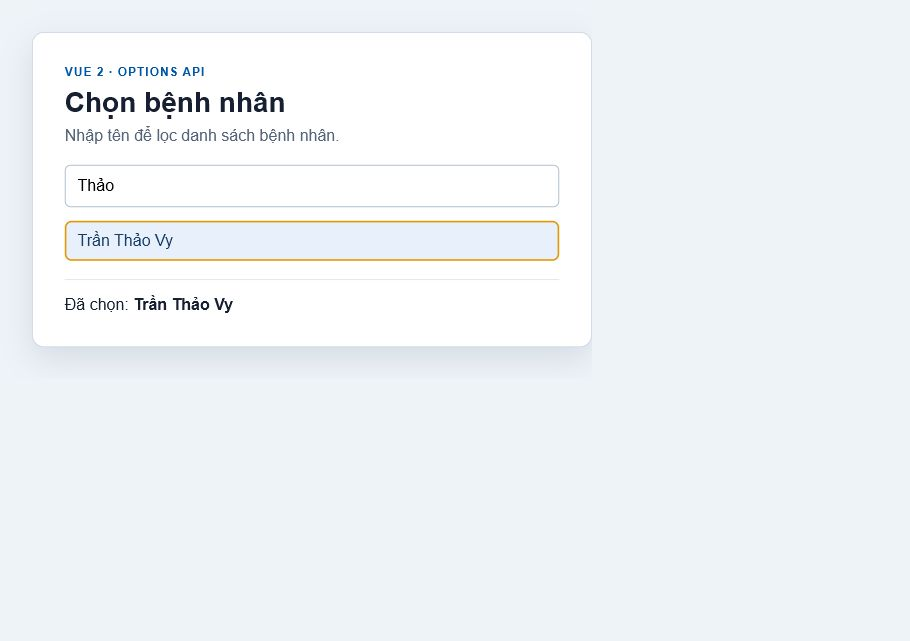
\includegraphics[width=0.64\textwidth,trim=0 270 280 0,clip]
  {../../assets/code-output/vue2-patient-picker-output.png}
\captionof{figure}{Kết quả chạy component \texttt{PatientPicker} sau khi build}
\label{fig:vue2-code-output}
\end{center}

\Needspace{0.24\textheight}
\subsection{Phân biệt methods, computed và watch}

\textbf{Tác vụ phụ} (side effect) là hành động không chỉ trả về một giá trị, chẳng
hạn gọi API, ghi bộ nhớ trình duyệt hoặc sửa state khác.

{\small
\begin{longtable}{|>{\raggedright\arraybackslash}p{0.18\textwidth}|
                  >{\raggedright\arraybackslash}p{0.34\textwidth}|
                  >{\raggedright\arraybackslash}p{0.38\textwidth}|}
\caption{Phân biệt methods, computed và watch}\label{tab:vue-options}\\
\hline
\textbf{Option} & \textbf{Bản chất} & \textbf{Ví dụ phù hợp} \\
\hline
\texttt{methods} & Hàm chạy mỗi lần được gọi; có thể thay đổi state hoặc phát sự kiện. & Xử lý click, gửi biểu mẫu hoặc gọi một hành động rõ ràng. \\
\hline
\texttt{computed} & Giá trị suy ra được lưu lại; chỉ tính lại khi state hoặc prop đã đọc bên trong thay đổi. & Danh sách đã lọc, tổng tiền hoặc trạng thái nút dựa trên nhiều trường dữ liệu. \\
\hline
\texttt{watch} & Theo dõi một giá trị và chạy tác vụ phụ khi giá trị đó đổi. & Gọi API tìm kiếm sau khi người dùng ngừng nhập trong một khoảng ngắn, ghi log hoặc đồng bộ với hệ thống bên ngoài. \\
\hline
\end{longtable}
}

Vì computed nên chỉ mô tả giá trị suy ra, tác vụ phụ thuộc về method hoặc watch. Nếu
có thể biểu diễn một giá trị bằng
computed thì không cần dùng watch để chép dữ liệu từ chỗ này sang chỗ khác
\cite{vue2-computed}.

\subsection{Cơ chế reactivity và cập nhật DOM}

Khi một đối tượng Vue 2 được tạo, Vue duyệt các thuộc tính đã khai báo trong
\texttt{data} và chuyển mỗi thuộc tính thành getter/setter bằng
\texttt{Object.defineProperty}:

\begin{itemize}
  \item \textbf{getter} chạy khi code đọc thuộc tính;
  \item \textbf{setter} chạy khi code gán giá trị mới cho thuộc tính;
  \item \textbf{dependency} là thuộc tính mà giao diện đã đọc và phụ thuộc vào;
  \item \textbf{watcher} là đối tượng theo dõi các dependency của component và được
  thông báo khi một dependency thay đổi.
\end{itemize}

Luồng cập nhật giao diện diễn ra theo thứ tự trong \figref{fig:vue-render-flow}:

\begin{center}
\resizebox{0.90\textwidth}{!}{\begin{tikzpicture}[
  node distance=3.2mm,
  every node/.style={font=\scriptsize,align=center},
  flowbox/.style={draw,rounded corners=1.5mm,minimum height=25mm,minimum width=20.5mm,text width=18mm,thick},
  number/.style={circle,fill=orange!80!black,text=white,font=\scriptsize\bfseries,inner sep=1.4mm},
  arrow/.style={-{Latex[length=1.8mm]},thick,draw=orange!80!black}
]
\node[flowbox,fill=orange!12,draw=orange!70!black] (s1) {State\\thay đổi};
\node[flowbox,fill=orange!8,draw=orange!70!black,right=of s1] (s2) {Getter/setter\\của Vue 2\\phát hiện};
\node[flowbox,fill=green!12,draw=green!55!black,right=of s2] (s3) {Watcher\\được\\thông báo};
\node[flowbox,fill=blue!10,draw=blue!55,right=of s3] (s4) {Render\\function\\chạy lại};
\node[flowbox,fill=violet!10,draw=violet!60,right=of s4] (s5) {Tạo\\Virtual DOM\\mới};
\node[flowbox,fill=blue!8,draw=blue!55,right=of s5] (s6) {So sánh diff\\và tạo\\bản vá patch};
\node[flowbox,fill=green!12,draw=green!55!black,right=of s6] (s7) {DOM thật / UI\\được cập nhật};

\foreach \a/\b in {s1/s2,s2/s3,s3/s4,s4/s5,s5/s6,s6/s7}
  \draw[arrow] (\a) -- (\b);

\node[number,above=2mm of s1] (n1) {1};
\node[number,above=2mm of s2] (n2) {2};
\node[number,above=2mm of s3] (n3) {3};
\node[number,above=2mm of s4] (n4) {4};
\node[number,above=2mm of s5] (n5) {5};
\node[number,above=2mm of s6] (n6) {6};
\node[number,above=2mm of s7] (n7) {7};

\node[draw=orange!70!black,dashed,rounded corners=1.5mm,below=7mm of s2,text width=43mm,minimum height=12mm]
  (detectnote) {Vue 2 dùng getter/setter để biết dependency nào đã thay đổi};
\draw[dashed,-{Latex[length=1.6mm]},draw=orange!70!black]
  (s2.south) -- (detectnote.north);

\node[draw=green!55!black,rounded corners=1.5mm,fill=green!8,below=7mm of s6,text width=50mm,minimum height=12mm,font=\small\bfseries,text=green!45!black]
  (resultnote) {Chỉ phần giao diện chịu ảnh hưởng được cập nhật};
\draw[dashed,-{Latex[length=1.6mm]},draw=green!55!black]
  (s7.south) -- (resultnote.north east);
\end{tikzpicture}
}
\captionof{figure}{Luồng Vue 2 ghi nhận thay đổi và cập nhật DOM}
\label{fig:vue-render-flow}
\end{center}

Template được biên dịch thành \textbf{hàm dựng giao diện} (render function). Khi watcher chạy lại, hàm
này tạo một cây \textbf{Virtual DOM}, tức biểu diễn JavaScript nhẹ của giao diện.
Vue thực hiện \textbf{diff} để so sánh cây mới với cây trước, sau đó \textbf{patch}
những thay đổi cần thiết vào DOM thật. Cách này tránh xây lại toàn bộ trang mỗi khi
một giá trị đổi.

Vue không cập nhật DOM ngay sau từng phép gán. Các watcher được đưa vào một hàng đợi;
nếu cùng watcher bị kích hoạt nhiều lần trong một lượt xử lý JavaScript, Vue chỉ giữ
một lần. Lượt xử lý kế tiếp gọi là \textbf{tick}; khi đó Vue xử lý hàng đợi và cập
nhật DOM. Khi code cần đọc
DOM sau cập nhật, dùng \texttt{await this.\$nextTick()}
\cite{vue2-instance,vue2-reactivity}.

\subsection{Giới hạn reactivity với object và array}

Vue 2 tạo getter/setter cho các thuộc tính tồn tại lúc đối tượng khởi tạo. Nếu thêm
một thuộc tính mới bằng phép gán thông thường, Vue không có setter cho thuộc tính đó
nên không biết phải thông báo watcher. \texttt{\$set} vừa thêm thuộc tính vừa đăng ký nó
vào hệ thống reactivity:

\Needspace{0.14\textheight}
\begin{lstlisting}
// Sai neu "note" chua ton tai luc khoi tao:
this.patient.note = 'VIP'

// Dung:
this.$set(this.patient, 'note', 'VIP')
\end{lstlisting}

Tương tự, Vue 2 không phát hiện chắc chắn phép gán trực tiếp theo index của array.
Dùng \texttt{\$set} hoặc một phương thức biến đổi mảng mà Vue đã bọc, chẳng hạn
\texttt{splice}:

\Needspace{0.10\textheight}
\begin{lstlisting}
this.$set(this.rows, index, updatedRow)
// hoac:
this.rows.splice(index, 1, updatedRow)
\end{lstlisting}

Cách đơn giản nhất vẫn là khai báo trước cấu trúc chính của state trong \texttt{data};
\texttt{\$set} dùng cho trường hợp thực sự cần thêm thuộc tính động
\cite{vue2-reactivity}.

\Needspace{0.14\textheight}
\section{Kết luận}

\begin{enumerate}
  \item Parallel phù hợp với phép tính CPU đủ nặng, có thể chia thành các phần tương
  đối độc lập và chỉ nên áp dụng sau khi so sánh với bản tuần tự. Từ .NET 6,
  \texttt{Parallel.ForEachAsync} bổ sung cách xử lý collection bằng hàm bất đồng bộ
  với số thao tác đồng thời được giới hạn.

  \item Background Job có thể triển khai bằng \texttt{IHostedService},
  \texttt{BackgroundService} hoặc mẫu project Worker Service. .NET 6 thay đổi cách
  Host xử lý lỗi chưa được bắt và bổ sung \texttt{PeriodicTimer}; .NET 8 bổ sung
  \texttt{TimeProvider} và các mốc vòng đời chi tiết hơn. Khi cần lưu job, tự động thử lại hoặc
  lịch phức tạp, cần cân nhắc Hangfire, Quartz.NET hay một hàng đợi bền vững.

  \item Vue 2 tổ chức component bằng Options API, liên kết template với state qua
  directive, props và event. Khi state thay đổi, hệ thống reactivity lên lịch dựng
  Virtual DOM mới, so sánh với cây trước và cập nhật phần DOM thật bị ảnh hưởng.
\end{enumerate}


\printbibliography[title={Tài liệu tham khảo}]

\end{document}
